\section{Building for Development}
\label{sec:developer:build}

For those less familiar with building software from source and using
Git for version control, we recommend using the PyLith developer
binary. This is a special binary that contains binary versions of all of the PyLith
dependencies except for spatialdata and PETSc. Those two dependencies
and PyLith are downloaded from the Git repositories, configured, and
built from source using a utility script. See Section
\vref{sec:developer:binary} for detailed instructions.

For those comfortable building from source and using Git for version
control, we recommend using the PyLith Installer utility (see Section
\vref{sec:developer:installer}) to build PyLith and its dependencies from
source.

% ------------------------------------------------------------------------------
\subsection{Developer Workflow}

We use the Git version control system \url{https://git-scm.com} with a
central GitHub repository \url{https://github.com/geodynamics/pylith}
for development. We will refer to this central repository as the
\gitbranch{geodynamics/pylith} repository. Only the PyLith maintainers
have write access to the \url{geodynamics/pylith} repository; everyone
else is limited to read access.

Currently, the PyLith maintainers use the
\href{https://www.atlassian.com/git/tutorials/comparing-workflows/gitflow-workflow}{Gitflow
  Workflow}, which is a variation, of the
\href{https://www.atlassian.com/git/tutorials/comparing-workflows/feature-branch-workflow}{Feature
  Branch Workflow} . New features are added on individual branches and
merged to specific shared branches.

At any given time there are three main shared Git branches:
\begin{description}
\item[\gitbranch{master}] The \gitbranch{master} branch is the
  stable development branch. We generally start new development by
  creating branches from this branch. Releases are created when the
  \gitbranch{master} branch has accumulated a desired set of features.
\item[\gitbranch{maint}] The \gitbranch{maint} branch is the
  maintenance branch for the current release. Bug fixes are pushed
  to this branch and merged to the \gitbranch{master} as
  appropriate. Upon a new release, the \gitbranch{master} branch is
  merged into the \gitbranch{maint} branch.
\item[\gitbranch{next}] The \gitbranch{next} is used to test
  integration of development branches. The PyLith maintainers test
  integration of new features they are implementing by merging to
  this branch, before merging them to the \gitbranch{master}
  branch.
\end{description}

Developers outside the PyLith maintainers follow the
\href{https://www.atlassian.com/git/tutorials/comparing-workflows/forking-workflow}{Forking
  Workflow} illustrated in
Figures~\vref{fig:developer:git:repositories}
and~\vref{fig:developer:git:branch}. Each developer forks the
\gitbranch{geodynamics/pylith} repository so that they have a copy of
the repository for their changes. Each new, independent feature you
develop should be done in a separate branch. Large feature
contributions should be broken up into multiple phases, where each
phase provides a working version that passes all of its tests. Each
phase corresponds to a separate branch that is merged back into the
\gitbranch{geodynamics/pylith} repository (usually the
\gitbranch{master} branch) via a
\href{https://help.github.com/articles/about-pull-requests/}{pull
  request} when it is completed.

\begin{figure}[htbp]
  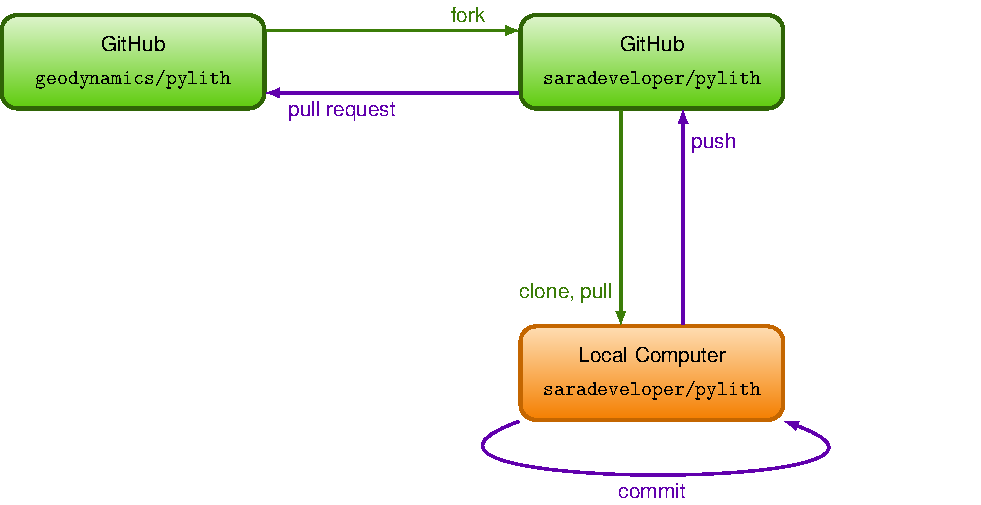
\includegraphics[scale=0.7]{developer/figs/gitworkflow_repositories}
  \caption{Overview of repositories for the Git forking workflow used in PyLith
    development. The main repository is the
    \filename{geodynamics/pylith} at GitHub. Developers create a fork
    of that repository under their own GitHub account (e.g.,
    saradeveloper), which is cloned to their local computer. Changes
    and additions to the code are committed to the repoisitory on the
    local computer, which are pushed to the developer's GitHub
    account. Once a development task is completed, a developer is
    encouraged to contribute the changes and additions to the main
    repository.}
  \label{fig:developer:git:repositories}
\end{figure}

\begin{figure}[htbp]
  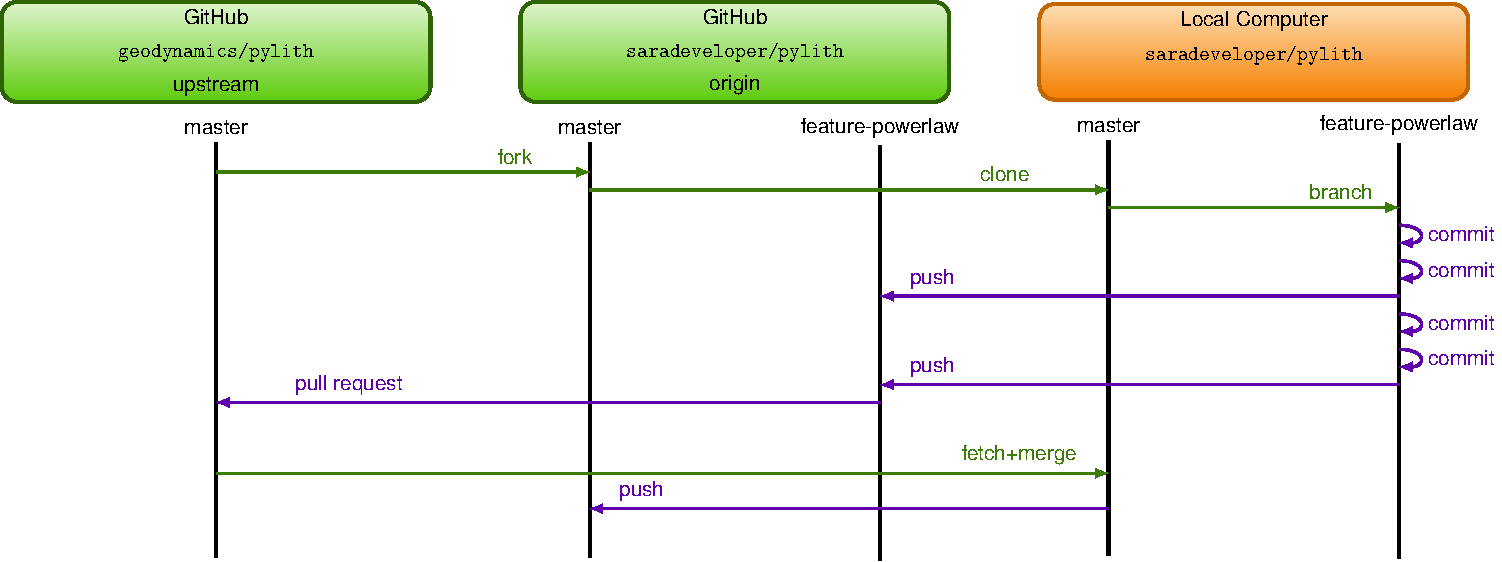
\includegraphics[scale=0.7]{developer/figs/gitworkflow_branch}
  \caption{Overview of repositories and branches for the Git forking
    workflow used in PyLith development. From the \gitbranch{master}
    branch on their local machine, a developer creates a feature
    branch, e.g., \gitbranch{feature-powerlaw}, to complete a single
    task such as adding a feature, fixing a bug, or making an
    improvement to the documentation. The developer will likely break
    up the changes into several steps, which as saved locally as
    commits. The commits may be pushed to the developer's repository
    on GitHub for backup or syncing on multiple computers. Once the
    task is completed, the developer submits a pull request to have
    the changes merged to the master branch on the community
    repository. Once the pull request is merged, the developer updates
    her own master branch on her local computer from the community
    repository and pushes the changes to her GitHub repository.}
  \label{fig:developer:git:branch}
\end{figure}

The PyLith maintainers would prefer to use the
\href{https://www.atlassian.com/git/tutorials/comparing-workflows/forking-workflow}{Forking
  Workflow} for all development, but this requires multiple dedicated
maintainers to review each other's code.

There are two steps to setting up a copy of the PyLith repository that
you can use for development under the Forking Workflow:
\begin{enumerate}
\item Create a GitHub account.
\item Fork the \gitbranch{geodynamics/pylith} repository.

  This will create a copy of the PyLith repository in your GitHub
  account. You can make changes to this copy and when you are ready to
  contribute changes back to the \gitbranch{geodynamics/pylith}
  repository you will create a pull request.
\end{enumerate}

\tip{We recommend adding your SSH public key to your GitHub account. See
\href{https://help.github.com/articles/connecting-to-github-with-ssh/}{GitHub Help: Connecting To GitHub with SSH} for
more information. This provides additional security and eliminates the need to enter your username and password
whenenver you push to your repository. For additional security consider setting up your GitHub account to use two-factor
authentication. See
\href{https://help.github.com/articles/securing-your-account-with-two-factor-authentication-2fa/}{GitHub Help: Securing
your account with two-factor authentication}.}

% ------------------------------------------------------------------------------
\subsection{Developer Binary}

\todo{brad}{Add this section when the developer binary is created.}

% ------------------------------------------------------------------------------
\subsection{PyLith Installer for Development}

The PyLith Installer utility can be used to build PyLith and all of
its dependencies from source. There are several configure arguments
relavant to using the installer for development:
\begin{description}
\item[\commandline{-{}-with-pylith-repo=URL}] Clone the PyLith source
  code from this URL. The URL corresponds to your fork of the PyLith
  repository. If you are accessing GitHub via SSH, the URL usually has
  the form \url{git@github.com:YOUR_GITHUB_USERNAME/pylith.git}. If
  you are accessing GitHub via HTTPS, the URL usually has the form
  \url{https://github.com/YOUR_GITHUB_USERNAME/pylith.git}. The
  default URL is the \gitbranch{geodynamics/pylith} repository,
  \url{https://github.com/geodynamics/pylith.git}.
\item[\commandline{-{}-with-pylith-git=BRANCH}] Build the
  \gitbranch{BRANCH} of PyLith. If you are just starting development
  and have not created any feature branches, then use the
  \gitbranch{knepley/feature-petsc-fe} branch.
\item[\commandline{-{}-with-spatialdata-repo=URL}] Clone the
  spatialdata source code from this URL. The default is the
  \gitbranch{geodynamics/spatialdata} repository,
  \url{https://github.com/geodynamics/spatialdata.git}. You do not
  need to change this unless you want to contribute to development of
  the spatialdata library.
\end{description}

\todo{brad}{Update the name of the branch in the description of
  \commandline{-{}-with-pylith-git} to \gitbranch{master} when
  \gitbranch{knepley/feature-petsc-fe} has been merged.}

Other common configure arguments used when configuring for development
include:
\begin{description}
  \item[\commandline{-{}-enable-swig}] Build the SWIG library for
    building the Python/C++ interface.
  \item[\commandline{-{}-enable-pcre}] Build the PCRE library for use
    in SWIG.
  \item[\commandline{-{}-enable-debugging}] Use debugging (generate
    debugging symbols and use low-level optimization) when building
    spatialdata, PETSc, and PyLith.
\end{description}

\tip{For all development, we build with debugging turned on. By
  building in directories separate from the source code, we can build
  an optimized version for production runs in a different directory and
  use environment variables to select the desired build.}

\begin{shell}[Example PyLith Installer setup for development]
# Prerequisites:
#  * C/C++ compiler
#  * autotools
#  * fork of PyLith repository

# Set some variables to hold information about our installer setup.
# The PYLITH_REPO should be
# https://github.com/YOUR_GITHUB_USERNAME/pylith.git or
# git@github.com:YOUR_GITHUB_USERNAME/pylith.git
$ PYLITH_DIR=$HOME/pylith-developer
$ PYLITH_REPO=git@github.com:YOUR_GITHUB_USERNAME/pylith.git
$ PYLITH_BRANCH=knepley/feature-petsc-fe

# Create a top-level directory for PyLith.
$ mkdir -p $PYLITH_DIR
$ cd $PYLITH_DIR

# Clone the installer.
$ git clone --recursive https://github.com/geodynamics/pylith_installer.git

# Generate the configure script (must have autotools installed).
$ cd pylith_installer && autoreconf -if

# Create a build directory for the installer and configure the installer
$ cd $PYLITH_DIR && mkdir build && cd build
$ ../pylith_installer/configure \
    --with-pylith-git=$PYLITH_BRANCH \
    --with-pylith-repo=$PYLITH_REPO \
    --enable-debugging \
    --enable-mpi=mpich \
    --enable-pcre \
    --enable-swig \
    --with-fetch=curl \
    --with-make-threads=2 \
    --prefix=$PYLITH_DIR/dist

# Check the configure output to make sure it ran without errors and
# the configuration matches what you want.

# Setup your environment
$ source setup.sh

# Build the dependencies and PyLith
$ make
\end{shell}

% ------------------------------------------------------------------------------
\subsection{Keeping Your Fork in Sync with \gitbranch{geodyamics/pylith}}

See Figure~\vref{fig:developer:git:branch} for the diagram of the
workflow associated with these steps.

\subsubsection{Set the upstream repository (done once per computer)}
\label{sec:developer:set:upstream}

On each computer where you have the clone of your fork, you need to
create a link to the ``upstream'' repository. This allows you to keep
your repository in sync with the central repository.

\begin{shell}[Setting upstream repository]
# List the current remotes for your fork.
$ git remote -v
origin git@github.com/YOUR_GITHUB_USERNAME/pylith.git (fetch)
origin git@github.com/YOUR_GITHUB_USERNAME/pylith.git (push)

# Set the link to the remote upstream repository
$ git remote add upstream https://github.com/geodynamics/pylith.git

# Verify the upstream repository has been added.
$ git remote -v
origin git@github.com/YOUR_GITHUB_USERNAME/pylith.git (fetch)
origin git@github.com/YOUR_GITHUB_USERNAME/pylith.git (push)
upstream https://github.com/geodynamics/pylith.git (fetch)
upstream https://github.com/geodynamics/pylith.git (push)
\end{shell}

\subsubsection{Merging Updates from the Upstream Repository}
\label{sec:developer:merge:upstream}

Make sure all of your local changes have been committed or
\href{https://git-scm.com/docs/git-stash}{stashed}.

\begin{shell}[Syncing your fork]
# Update your local version of the upstream repository
$ get fetch upstream

# Check out the 'knepley/feature-petsc-fe' branch
$ git checkout knepley/feature-petsc-fe
Switched to branch 'knepley/feature-petsc-fe'

# Merge 'knepley/feature-petsc-fe' from upstream to your local clone.
$ git merge upstream/knepley/feature-petsc-fe

# If there are no conflicts, push the changes to your fork on GitHub.
$ git push

# If you need to update a local branch with changes from
# 'knepley/feature-petsc-fe', then checkout the branch and
# merge the local 'knepley/feature-petsc-fe' branch.
$ git checkout MY_USERNAME/feature-something-great
$ git merge knepley/feature-petsc-fe
\end{shell}

\subsection{Creating a New Feature Branch}
\label{sec:developer:create:branch}

Before creating a new feature branch, you should merge updates from
the upstream repository as described in Section~\vref{sec:developer:merge:upstream}.

\begin{shell}[Creating a feature branch]
# Start from the current development branch (usually 'master')
$ git checkout master

# Make sure it is up to date.
$ git pull

# Create branch from 'master', substituting appropriate names for
# USERNAME and BRANCH.
$ git checkout -b USERNAME/BRANCH
\end{shell}

\subsection{Staging, Committing, and Pushing Changes}
\label{sec:developer:commit}

The Git \commandline{add} and \commandline{commit} commands are used
to commit changes to a branch. A commit changes only the current
branch in the repository clone on your local machine. In order to
update your GitHub fork you need to \commandline{push} your
changes. See the Git documentation for details about these
commands. There are Git interfaces built into a number of editors and
integrated development environments (IDEs), and there are standalong
graphical user interfaces to Git.

\tip{If you have multiple branches, make sure you are on the correct
  branch before making commits.}

\subsection{Making Pull Requests}
\label{sec:developer:create:pull:request}

Once you have completed implementing and testing a new feature on a
branch in your fork and wish to contribute it back to the
\gitbranch{geodynamics/pylith} repository, you open a pull
request. See
\href{https://help.github.com/articles/about-pull-requests/}{GitHub
  Help: About pull requests} for more information.


% ------------------------------------------------------------------------------
\subsection{Rebuilding PETSc}

Updating and rebuilding PETSc is quite simple once it has been configured and built once before.

\begin{shell}[Updating and rebuilding PETSc]
# Change to PETSc source Directory
$ cd PETSC_SOURCE_DIRECTORY

# Get updates from PETSc repository.
$ git pull

# Reconfigure
$ arch-pylith/lib/petsc/conf/reconfigure-arch-pylith.py

# Rebuild
$ make

# Install
$ make install
\end{shell}

% ------------------------------------------------------------------------------
\subsection{Rebuilding PyLith}

\subsubsection{Overview}

Pylith uses the GNU Build System (autotools: autoconf, automake,
libtool) to configure and build. The configure settings are defined in
\filename{configure.ac} with additional macros in the \filename{m4}
directory. Note that the \filename{m4} directory is a Git submodule
corresponding to the \filename{geodynamics/autoconf} Git repository.

\subsubsection{Makefiles}

The PyLith \filename{configure} script uses automake to convert each
\filename{Makefile.am} file into a \filename{Makefile}. The
organization and content of the \filename{Makefile.am} file depends on
whether it is related to the C++ library, SWIG interface files, Python
modules, C++ unit tests, Python unit tests, or examples.

For the C++ library files within the \filename{libsrc} directory, the
\filename{libsrc/Makefile.am} contains the implementation files while
the header files are listed in the \filename{Makefile.am} file within
the underlying directories.

For the SWIG interface files within the \filename{modulesrc}
directory, the \filename{Makefile.am} file contains information on how
to build the SWIG Python module.

The Python modules use a single \filename{Makefile.am} file in
the \filename{pylith} directory.

Each test suite (C++ unit tests for each subpackage, Python unit tests
for each subpackage, and each suite of full-scale tests) use a single
\filename{Makefile.am}. These files define how the tests are built,
additional input files that should be included in the source
distribution, and temporary files that should be deleted.

Each suite of examples contains a \filename{Makefile.am} that defines
the files that are to be included in the source distribution. It also
defines which files are created and should be deleted upon
\commandline{make clean}.

\subsubsection{Build Targets}

Several build targets are defined to make it easy to rebuild/reinstall
PyLith rerun tests whenever the source code changes. Each target can
be run using \commandline{make TARGET} where \commandline{TARGET} is
one of the following:

\begin{description}
\item[all] Build.
\item[install] Build and install.
\item[check] Run all unit tests and full-scale automated tests.
\end{description}

\tip{On a machine with multiple cores, faster builds of the C++ code
  (library and C++ unit tests) are available using the
  \commandline{-jNTHREADS} command line argument, where
  \commandline{NTHREADS} is the number of cores to use. For example,
  \commandline{make -j16 all}.}

After modifying code, the C++ library, SWIG modules, and Python code need to be rebuilt and reinstalled before running a
PyLith simulation.

\begin{shell}[Rebuilding Pylith C++ library, SWIG modules, and Python modules]
# Change to top-level PyLith build directory.
$ cd PATH_TO_PYLITH_BUILD_DIRECTORY

# Rebuild and reinstall library using 8 threads.
$ make install -j8 -C libsrc

# Rebuild and reinstall modules
$ make install -C modulesrc

# Reinstall Python code
$ make install -C PyLith

# Reinstall everything using 8 threads to build library.
$ make install -j8
\end{shell}

When fixing a bug exposed by a C++ unit test, after changing C++ code, only the C++ library needs to be rebuilt before
running a C++ unit test.

\begin{shell}[Rebuilding Pylith C++ library and rerunning a C++ unit test]
# Change to top-level PyLith build directory.
$ cd PATH_TO_PYLITH_BUILD_DIRECTORY

# Rebuild library using 8 threads.
$ make -j8 -C libsrc

# Rerun boundary condition C++ unit tests.
$ make check -C unittests/libtests/bc
\end{shell}

Similarly, when fixing a bug exposed by a Python unit test, after changing Python code, only the Python modules need to
be reinstalled before running a Python unit test. If changes are also made to the C++ code, then the C++ library and modules
must be rebuilt and reinstalled before running a Python unit test.

\begin{shell}[Rebuilding Pylith Python modules and rerunning a Python unit test]
# Change to top-level PyLith build directory.
$ cd PATH_TO_PYLITH_BUILD_DIRECTORY

# Reinstall PyLith Python modules.
$ make install -C pylith

# Rerun boundary condition Python unit tests.
$ make check -C unittests/pytests/bc
\end{shell}


% End of file
